\subsection{Understanding Timeline Interfaces}\label{sec:client-timeline}

A \emph{timeline interface} assigns each input or output of a hardware module a \emph{timeline type}~\cite{nigam_modular_2023} that specifies the clock-cycle intervals during which the corresponding signal is required or available.
Such information is important for hardware developers to \emph{understand} how to correctly use a module.
However, Chisel does not provide a type system with timeline types that explicitly encode this temporal information.
Consequently, developers must typically obtain it from documentation, build scripts, or, in the worst case, the module's implementation.
As a final client analysis built on top of \tia, we develop \emph{timeline interface analysis}, which automatically computes an approximation of a module's actual timeline interface.
Although our analysis cannot automatically and precisely equip existing Chisel codebases with the informative timeline type system, we believe that even an approximate timeline interface can still be help helpful for developers to \emph{understand} the temporal behavior of a module by making it more explicit.
We first illustrate the notion of a timeline interface through a simplified example and then describe how our timeline interface analysis approximates such interfaces from the temporal influence information computed by \tia.

\begin{figure}[tp]
    \hfill
    \begin{subfigure}[b]{.45\textwidth}
        \begin{subfigure}{\linewidth}
            \centering
            \begin{chisel}
class AU extends Module {
    val a         = Input(UInt(32.W))
    val b         = Input(UInt(32.W))
    val a_plus_b  = Output(UInt(32.W))
    val a_plus_2b = Output(UInt(32.W))
    // --- Compute a + b ---
    val reg_a  = Reg(UInt(32.W))
    val reg_b  = Reg(UInt(32.W))
    reg_a     := a
    reg_b     := b
    a_plus_b  := reg_a + reg_b
    // --- Compute a + 2b ---
    val reg_a_plus_b = Reg(UInt(32.W))
    val reg_reg_b    = Reg(UInt(32.W))
    reg_a_plus_b := a_plus_b
    reg_reg_b    := reg_b
    a_plus_2b := reg_a_plus_b + reg_reg_b
}
            \end{chisel}
            \caption{A simple Chisel arithmetic unit \texttt{AU}.}
            \label{fig:timeline-code}
        \end{subfigure}

        \vspace{1ex}

        \begin{subfigure}{\linewidth}
            \centering
            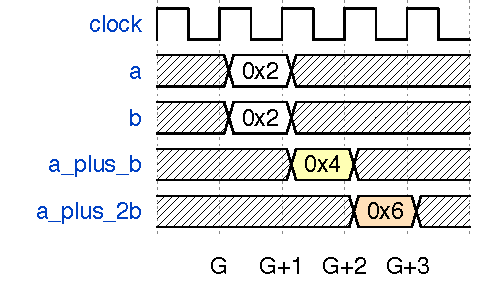
\includegraphics[width=\linewidth,clip,trim=15 15 12 0]{figures/timeline-waveform}
            \caption{Waveform illustrating the temporal behavior of \texttt{AU}, where $G$ denotes any clock-cycle time.}
            \label{fig:timeline-waveform}
        \end{subfigure}


    \end{subfigure}
    \hfill
    \begin{subfigure}[b]{.5\textwidth}
        \begin{subfigure}{\linewidth}
            \centering
            \[
            \begin{aligned}
                \forall G.\ & \textpurple{\mathtt{a}} \in [G, G+1) \wedge \textpurple{\mathtt{b}} \in [G, G+1) \\
                \Rightarrow\ & \textblue{\mathtt{a\_plus\_b}} \in [G+1, G+2)\\
                & \wedge \textblue{\mathtt{a\_plus\_2b}} \in [G+2, G+3)
            \end{aligned}
            \]
            \caption{The timeline interface of \texttt{AU}, expressed as a proposition about its temporal behavior, where $x \in [G+i,G+j)$ means that $x$ is valid from clock cycle $G+i$ through, but not including, clock cycle $G+j$.}
            \label{fig:timeline-interface}
        \end{subfigure}

        \vspace{1ex}

        \begin{subfigure}{\linewidth}
            \centering
            \footnotesize
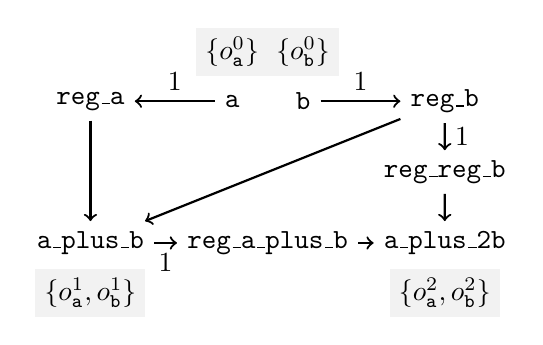
\begin{tikzpicture}[scale=.9,thick]
    \node (a) at (2, 0) {$\textpurple{\mathtt{a}}$};
    \node (b) at (3, 0) {$\textpurple{\mathtt{b}}$};
    \node (ra) at (0, 0) {$\mathtt{reg\_a}$};
    \node (rb) at (5, 0) {$\mathtt{reg\_b}$};
    \node (rrb) at (5, -1) {$\mathtt{reg\_reg\_b}$};
    \node (ab) at (0, -2) {$\textblue{\mathtt{a\_plus\_b}}$};
    \node (rab) at (2.5, -2) {$\mathtt{reg\_a\_plus\_b}$};
    \node (a2b) at (5, -2) {$\textblue{\mathtt{a\_plus\_2b}}$};

    \draw [->] (a) --node[above]{$1$} (ra);
    \draw [->] (ra) -- (ab);
    \draw [->] (rb) -- (ab);
    \draw [->] (b) --node[above]{$1$} (rb);
    \draw [->] (rb) --node[right]{$1$} (rrb);
    \draw [->] (ab) --node[below]{$1$} (rab);
    \draw [->] (rab) -- (a2b);
    \draw [->] (rrb) -- (a2b);

    \node[fill=gray!10] at (2, .7) {$\{o_{\mathtt{a}}^0\}$};
    \node[fill=gray!10] at (3, .7) {$\{o_{\mathtt{b}}^0\}$};

    \node[fill=gray!10] at (0, -2.7) {$\{o_{\mathtt{a}}^1, o_{\mathtt{b}}^1\}$};
    \node[fill=gray!10] at (5, -2.7) {$\{o_{\mathtt{a}}^2, o_{\mathtt{b}}^2\}$};
\end{tikzpicture}

            \caption{\tia results showing the temporal influences of \texttt{AU}'s inputs (purple) on its outputs (blue).}
            \label{fig:tia-timeline}
        \end{subfigure}

        \vspace{1ex}

        \begin{subfigure}{\linewidth}
            For all $G$, let $I_G(x)$ be the \emph{minimal} interval $[G+i, G+j)$ that \emph{contains}
            \[
            \left\{G + i \mid \exists p \in \ports.\ o_p^i \in \absT(x)\right\}.
            \]
            We observe
            \[
            \textblue{\mathtt{a\_plus\_b}} \in [G + 1, G + 2) \subseteq I_G(\textblue{\mathtt{a\_plus\_b}})
            \]
            and
            \[
            \textblue{\mathtt{a\_plus\_2b}} \in [G + 2, G + 3) \subseteq I_G(\textblue{\mathtt{a\_plus\_2b}}).
            \]
            \caption{An observation guiding timeline interface analysis.}
            \label{fig:timeline-observe}
        \end{subfigure}
    \end{subfigure}
    \hfill
    \caption{A motivating example for timeline interface analysis.}
\end{figure}

\paragraph{Example of a Timeline Interface}

Figure~\ref{fig:timeline-code} shows a simple Chisel arithmetic unit \texttt{AU} (Line~1) with inputs \texttt{a} and \texttt{b} (Lines~2--3) and outputs \texttt{a\_plus\_b} and \texttt{a\_plus\_2b} (Lines~4--5).
The module takes one clock cycle to compute $\mathtt{a}+\mathtt{b}$ and produces the result at \texttt{a\_plus\_b} (Lines~6--11).
It then takes another cycle to compute $\mathtt{a}+2\mathtt{b}$ and produces the result at \texttt{a\_plus\_2b} (Lines~12--17).
Figure~\ref{fig:timeline-waveform} visualizes this temporal behavior, where $G$ denotes a generic clock-cycle time at which the inputs are provided to \texttt{AU}.

Figure~\ref{fig:timeline-interface} summarizes this behavior as a timeline interface.
Specifically, if the user provides \texttt{a} and \texttt{b} during $[G,G+1)$, then \texttt{a\_plus\_b} becomes available during $[G+1,G+2)$, while \texttt{a\_plus\_2b} becomes available during $[G+2,G+3)$.
With this timeline interface, a user can \emph{understand} when the outputs of \texttt{AU} become available without inspecting its implementation.

\paragraph{Insights of Timeline Interface Analysis}

Figure~\ref{fig:tia-timeline} shows the \tia results for the \texttt{AU} module in Figure~\ref{fig:timeline-code}, focusing on its inputs and outputs.
We observe that \texttt{a\_plus\_b} can be influenced by an input only after one cycle, whereas \texttt{a\_plus\_2b} can be influenced by an input only after two cycles.
Assuming that both \texttt{a} and \texttt{b} are provided during $[G,G+1)$, this temporal influence information implies that \texttt{a\_plus\_b} becomes available during $[G+1,G+2)$ and \texttt{a\_plus\_2b} during $[G+2,G+3)$.
These intervals coincide with the timeline interface shown in Figure~\ref{fig:timeline-interface}.
The observation is summarized in Figure~\ref{fig:timeline-observe}.

Guided by this observation, we generalize the outputs of \texttt{AU} to an arbitrary output $x\in\variables$.
For each output $x$, our \emph{timeline interface analysis} infers the minimal interval $[G+i_x,G+j_x)$ such that
\[
\left\{G + i \mid \exists p \in \ports.\ o_p^i \in \absT(x)\right\} \subseteq [G+i_x, G+j_x).
\]
The resulting approximated timeline interface is therefore
\[
\forall G.\ (\forall p.\ p \in [G, G+1)) \Rightarrow (\forall x.\ x \in [G + i_x, G + j_x)).
\]


Compared with the precise timeline type system of~\cite{nigam_modular_2023}, which requires timeline information to be explicitly annotated in the hardware design, our timeline interface analysis is fully automated at the cost of:
\begin{enumerate}[leftmargin=*]
    \item
    \emph{Input Timeline Assumption.}
    Because Chisel designs do not provide timeline type annotations, we therefore assume that every input port $p$ is available during $[G,G+1)$.
    We made this assumption because we observed that most inputs are annotated with the timeline type $[G,G+1)$ in the benchmarks evaluated by~\cite{nigam_modular_2023}.
    Thus, although this assumption does not cover arbitrary timeline interfaces, it applies to a practically relevant class of modules.
    \item
    \emph{Over-Approximation.}
    The inferred timeline intervals may be larger than the corresponding precise timeline types and therefore contain false positives.
    This imprecision originates from the underlying \tia analysis, which soundly considers all TIG paths without distinguishing whether they are jointly feasible (which is termed \emph{path-insensitive} in software static analysis).
    A more path-sensitive formulation of \tia could potentially reduce such false positives and consequently produce tighter timeline interfaces, which we may explore in the future work.
\end{enumerate}
It is important to note that our timeline interface analysis is \emph{orthogonal} to the timeline type system of~\cite{nigam_modular_2023}, rather than a competitor to it.
The two approaches serve fundamentally different purposes:
timeline types help developers specify and check intended temporal behavior, whereas our analysis helps developers understand existing temporal behavior.
To be specific, the timeline type system is a \emph{specification and checking mechanism}:
developers explicitly annotate their hardware design with timeline types to express their temporal intentions, and the type system checks whether these annotations are safe (i.e., consistent) throughout the design.
In contrast, our timeline interface analysis is a \emph{design-understanding mechanism}:
given an unfamiliar hardware module without timeline types, a developer can apply the analysis to automatically obtain an approximate timeline interface and more easily understand how to use the module.
